
\section{Introduction}
\subsection{Supertree Estimation}
Supertree estimation is an important phylogenetic problem. Methods for supertree estimation take as input a set of source trees and output a single supertree. Each input tree is on a subset of the entire taxon set, and discrepancies between the input trees result only from estimation error, not from sources of true tree heterogeneity like incomplete lineage sorting or horizontal gene transfer \cite{warnow2018supertree}. Supertree methods are commonly used in phylogenetic analyses (e.g. \cite{cisneros2019phylogenetic,mcmahon2006phylogenetic,wojciechowski2000molecular,kennedy2002seabird}), and development of supertree methods is an area of active research \cite{superfine,mrl,fastrfs,fleischauer2017bad}.

Supertree methods are used in two contexts: traditionally, they are used to combine species trees from separate analyses into one large tree. They can also be used to scale up species tree analyses on multi-locus data with gene tree heterogeneity due to incomplete lineage sorting (ILS) \cite{maddison1997gene} when used as a component of divide and conquer methods \cite{warnow2019divide, dactal}. In these methods, a large species tree dataset is split into several small overlapping taxon sets. An accurate species tree estimation method is run on each of these small subsets, and then a supertree method is used to combine the subsets into a tree on the entire taxon set. Then, this process is repeated, with the tree from the previous iteration used to guide the new decomposition of the taxon set into overlapping subsets. Iterative divide and conquer methods enable the use of relatively slow methods, including computationally expensive Bayesian methods, on large phylogenomic datasets.

Upcoming cutting edge phylogenomic analyses will involve tens of thousands of taxa \cite{koepfli2015genome, zhang2015genomics}. Computing trees on these datasets will require scaling accurate methods beyond what is currently possible, and divide and conquer methods are a promising technique for this. However, these require supertree methods that can run on datasets with tens of thousands of taxa. 

Three different kinds of methods are currently used for supertree estimation \cite{warnow2018supertree}. Bipartition-based methods, including Matrix Representation with Parsimony (MRP) \cite{ragan1992phylogenetic}, Matrix Representation with Likelihood (MRL) \cite{mrl}, Bad Clade Deletion \cite{fleischauer2017bad}, Robinson-Foulds supertrees \cite{bansal2010robinson} (such as FastRFS \cite{fastrfs}, PluMiST \cite{plumist}, and MulRF \cite{mulrf}), and likelihood-based supertrees \cite{steel2008maximum}, use the distribution of bipartitions in the source trees to estimate a supertree. 

Quartet-based methods, most notably ASTRAL \cite{ASTRAL,ASTRAL-II,ASTRAL-III,ASTRAL-MP}, are typically used for species tree estimation from multi-locus gene trees with heterogeneity due to ILS, but can also be used for supertree estimation. They find a tree that maximizes the number of quartets (induced four-leaf trees) shared with the input trees. 

Distance-based methods, including neighbor joining \cite{saitou1987neighbor}, FastME \cite{lefort2015fastme}, and ASTRID \cite{vachaspati2015astrid}, are a third type of phylogenetic estimation method that can be used for supertrees. These methods construct a distance matrix (i.e., a mapping from pairs of taxa to distances) or set of distance matrices from the input trees and construct a tree that has a distance matrix similar to the one from the input trees.

\subsection{ASTRID}

ASTRID \cite{vachaspati2015astrid} is a method for phylogenetic estimation originally based on NJst \cite{liu2011estimating} and developed as a species tree method. It calculates a distance matrix from each input tree, averages them together, and uses a distance-based estimation method like neighbor joining with BIONJ* \cite{phydstar} or minimum-evolution estimation with FastME \cite{lefort2015fastme} to compute a tree. It is a statistically consistent estimation method under the coalescent model \cite{maddison1997gene}, on datasets with gene tree heterogeneity due to ILS.

Typically, ASTRID uses the minimum-evolution distance method FastME to estimate the species tree. FastME is fast and gives accurate results in practice. However, it requires a distance estimate for each pair of taxa; in other words, a complete distance matrix without any missing entries. If the distance matrix has missing entries, the original version of ASTRID used a neighbor joining variant called BIONJ* to estimate the species tree from the distance matrix. In practice, this is slow and tends to produce inaccurate trees. 

In this paper, we present and test a new iterative approach to ASTRID when the distance matrix is missing entries. We evaluate this on biological and simulated datasets, including a very large simulated dataset with over 40,000 taxa.

\begin{figure*}[!htb]
    \centering
    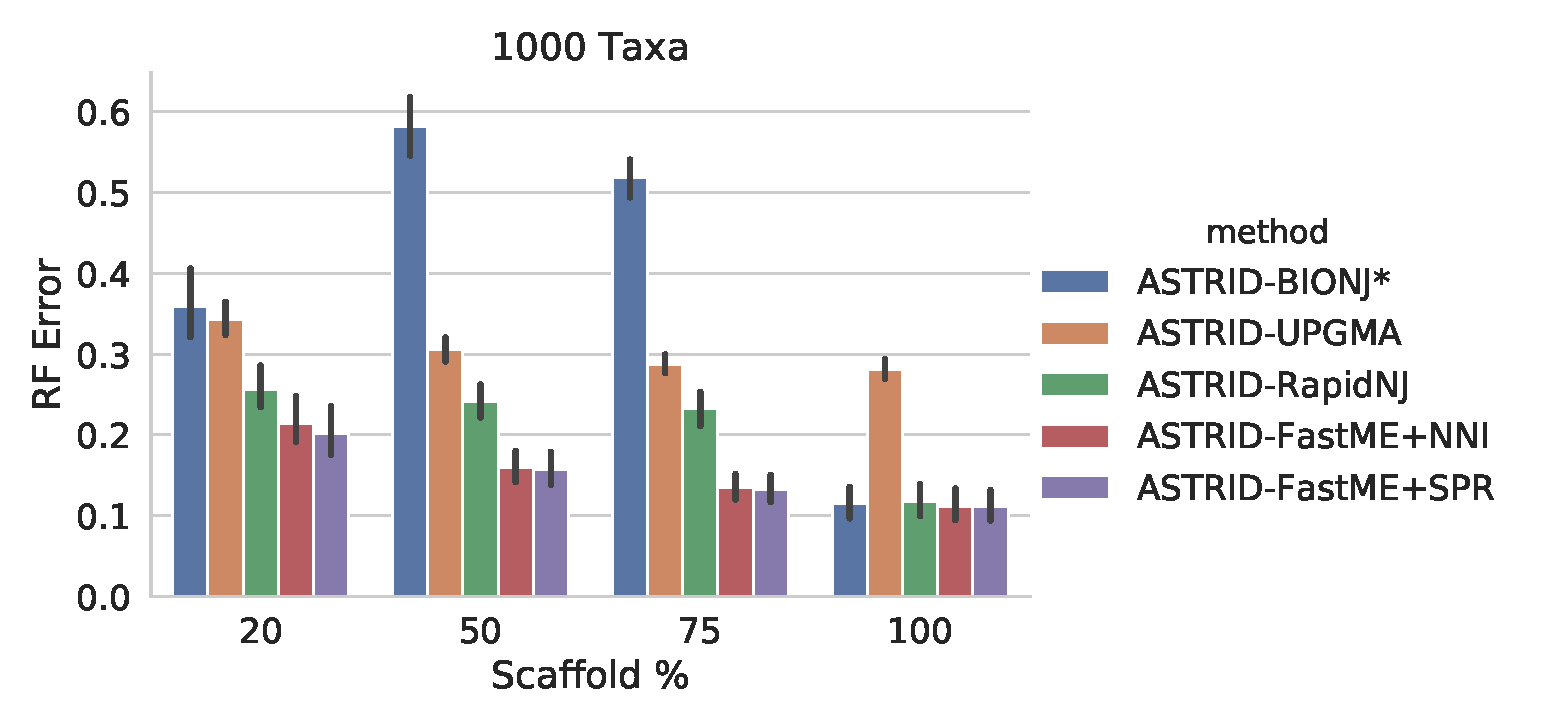
\includegraphics[width=\textwidth]{astrid-missing-figs/astrid-bionj-errs.eps}
    \caption[Error rates for ASTRID with BIONJ* and ASTRID with FastME using the UPGMA protocol]{Comparison of RF errors for ASTRID with BIONJ* and ASTRID with FastME using the UPGMA protocol. ASTRID-BIONJ* is used by the original version of ASTRID when the distance matrix is missing data. Results are shown on 1000-taxon SMIDgen data with 16 source trees. Data is averaged over 10 replicates.}
    \label{astrid-missing::fig:astrid-bionj-errs}
\end{figure*}

\section{Methods}
Previous versions of ASTRID used BIONJ* as a distance based species tree estimation method on datasets where ASTRID's distance method was missing entries.

BIONJ* is a modified version of neighbor joining. BIONJ \cite{gascuel1997bionj} applies a weighting scheme to the neighbor joining algorithm based on a simple model of variances in the distance matrix. This model, derived from the Jukes-Cantor model of sequence evolution \cite{jukes1969evolution}, predicts that the variance of a distance estimate between two taxa is proportional to the distance between those taxa. BIONJ* further extends BIONJ by allowing for distance matrices with missing taxa. This technique combines some straightforward modifications of the BIONJ algorithm with a set of heuristics to break ties at decision points within the algorithm.

This approach suffers from several issues. First, in some cases, the accuracy suffers substantially on these datasets when BIONJ* must be used. Second, the running time of BIONJ* is $O(n^3)$ in the number of taxa, and dominates the running time of ASTRID on larger datasets with high levels of missing data. Third, and somewhat less importantly, BIONJ* requires Java to be installed and configured appropriately on the user's computer, which can be challenging for the user. 

The improved version of ASTRID presented here retains the option to use BIONJ*, but adds a new iterative approach that mitigates all three of these issues. First, ASTRID uses a variant of UPGMA \cite{sokal1958statistical}, UPGMA*, which we have developed for this purpose, to quickly generate a (likely inaccurate) species tree. Then, it uses the UPGMA* tree to fill in the missing entries in the distance matrix, allowing for a fast and accurate method that requires a complete distance matrix to be run.


\subsection{UPGMA*}

We have developed a novel distance method, UPGMA*, which extends UPGMA so that it can be used on incomplete distance matrices. 

UPGMA and UPGMA* take as input an $n$ element taxon set $S$ and an $n\times n$ distance matrix $D$. They output a species tree $T$. 
UPGMA operates as follows:
\begin{enumerate}
    \item Initialize a forest data structure $F$ with $n$ independent elements corresponding to the $n$ taxa
    \item Initialize $n$ min-heap priority queues $Q_1,\ldots,Q_n$ that hold $<distance, taxon>$ pairs. 
    \item Initialize a map $M$ with $\langle taxon, taxon\rangle$ pairs as the keys and $distance$s as the values. 
    \item Mark each taxon as alive, and set the size of each taxon to $1$
    \item For each pair of taxa $i,j$, add $\langle D[i,j], j\rangle$ to $Q_i$ and $\langle D[i,j], i\rangle$ to $Q_j$
    \item For each pair of taxa $i,j$, add $\langle i, j\rangle \rightarrow D[i,j]$ to $M$
    \item While $F$ is disconnected:
    \begin{enumerate}
        \item For each priority queue $Q_i$ where $i$ is marked alive:
        \begin{enumerate}
            \item Pop elements from $Q_i$ until the top element has a taxon marked alive
            \item Let $best_i$ be the top element of $Q_i$
        \end{enumerate}
        \item Let $Q_x$ be the priority queue with the smallest top element. That top element is $best_x = \langle d_{min}, y\rangle$
        \item Create a new taxon $xy$ and mark it alive. Let $size(xy) = size(x) + size(y)$
        \item Mark taxa $x$ and $y$ as dead
        \item Add $xy$ to $F$ and set its children as $x$ and $y$
        \item Create a new priority queue $Q_{xy}$. 
        \item For each alive taxon $i$:
        \begin{enumerate}
            \item Let $d_{xy,i} = \frac{size(x) M[x, i] + size(y)M[y,i]}{size(x) + size(y)}$.
            \item Add $\langle xy, i \rangle \rightarrow d_{xy, i}$ to $M$
            \item Add $\langle d_{xy, i}, i \rangle$ to $Q_{xy}$. 
        \end{enumerate}
    \end{enumerate}
    \item Let $T$ be the sole tree in $F$. Return $T$.
\end{enumerate}

The overall asymptotic running time for this algorithm is $O(n^2\log n)$: in each of the $O(n)$ iterations, $O(n)$ items are added to priority queues. Each addition takes $O(\log n)$ time. Since each item can be removed from a priority queue at most once, the total time taken for both additions and removals from priority queues is $O(n^2\log n)$.

UPGMA* differs in a few ways that allow for distance matrices to contain missing elements. 

First, when the data structures are initialized, only taxon pairs where the distances are known are considered.

Second, when $d_{xy,i}$ is computed, if $M[x,i]$ is unknown, $d_{xy,i} = M[y,i]$, and if $M[y,i]$ is unknown, $d_{xy,i} = M[x, y]$. If both $M[x,i]$ and $M[y,i]$ are unknown, $d_{xy,i}$ is unknown, and the corresponding elements are not added to $M$ or $Q_{xy}$.

Third, if after removing dead elements, every priority queue is empty (and the forest is still disconnected), the distance matrix is disconnected; i.e. there are two disjoint subsets of taxa $S_1$ and $S_2$ such that $S_1 \cup S_2 = S$ and $\forall_{i \in S_1, j \in S_2}, D[i, j] $ is missing. In this case, UPGMA* picks an arbitrary pair of taxa to join and outputs a warning to the user.

These changes do not increase the asymptotic running time of UPGMA*. Since UPGMA is known to not be statistically consistent, UPGMA* is also not statistically consistent.

\subsubsection{Iterative protocol}

First, ASTRID calculates a distance matrix from the input trees. This matrix, $M_0$, may have missing entries. Then, UPGMA* is run, resulting in a tree $T_U$ that has a topological distance matrix $M_U$. Each missing entry in $M_0$ is replaced with the corresponding entry in $M_U$ to get the distance matrix $M_1$, which has no missing entries. Now, FastME (or another distance method) can be run on $M_1$ to get a tree $T_1$. The matrix from $T_1$, $M_1'$, can be used once again to fill in the missing entries in $M_0$ to get $M_2$, and FastME can again be run on this matrix. This procedure can be iterated further, and the final tree is the output.

\begin{figure*}[!htb]
    \centering
    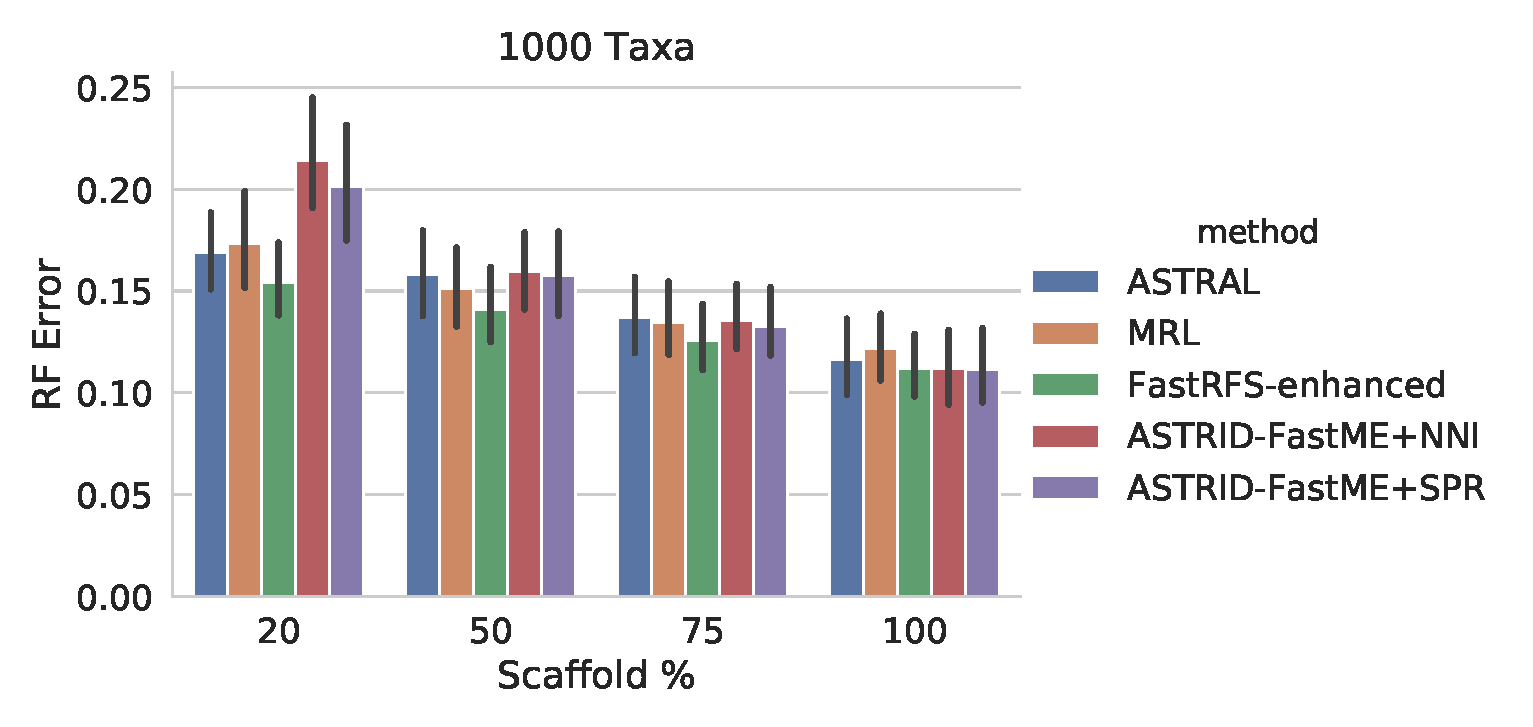
\includegraphics[width=\textwidth]{astrid-missing-figs/astral-errs.eps}
    \caption[RF errors for supertree methods and ASTRID variants with FastME using the UPGMA protocol]{Comparison of RF errors for supertree methods and ASTRID variants with FastME using the UPGMA protocol. Results are shown on 1000-taxon SMIDgen data with 16 source trees. Data is averaged over 10 replicates.}
    \label{astrid-missing::fig:astral-errs}
\end{figure*}

\subsection{Distance Methods}

ASTRID can use a variety of different distance methods to compute the species tree. The balanced minimum-evolution (BME) estimator in FastME is the default method used when the distance matrix is complete. Balanced minimum-evolution estimation has some theoretical similarities to neighbor joining \cite{gascuel2006neighbor}, but FastME is able to obtain more accurate results and run more quickly than standard neighbor joining implementations. FastME uses a taxon addition strategy, in contrast with the agglomerative approach used by neighbor joining, and then can improve its tree with nearest-neighbor interchanges (NNIs) and subtree prune-and-regraft moves (SPRs). 

BIONJ*, as discussed above, is a modification to the neighbor-joining algorithm that incorporates variance estimates for the elements in the distance matrix, and also is able to run on incomplete distance matrices.

RapidNJ \cite{simonsen2008rapid} is an implementation of neighbor joining designed to scale to extremely large datasets. It uses heuristics to significantly reduce the number of options considered in each iteration of the neighbor joining algorithm. In fact, while most distance methods require the entire distance matrix to fit into memory, RapidNJ is able to store most of the distance matrix on disk, paging portions into main memory only as needed \cite{simonsen2010inference}. While this has a negative impact on running time, it enables analyses of a size impossible with other methods.



\section{Experiments}

Previous studies of supertree methods \cite{fastrfs,smidgen} compared the performance of leading supertree and species tree methods, including ASTRID, on simulated and biological datasets. 
One study \cite{fastrfs} showed that ASTRID performed poorly in terms of accuracy and running time when the distance matrix was missing elements. For this paper, we replicated some of the analyses from those studies and also analyzed one newly simulated dataset.

\subsection{Datasets}

\subsubsection{Simulated SMIDgen datasets}
For this paper, we ran our improved version of ASTRID on SMIDgen datasets originally analyzed in \cite{smidgen} and also analyzed in \cite{fastrfs}. These simulated datasets had $100$, $500$, or $1000$ taxa. The $100$ taxon replicates had $6$ source trees, the $500$ taxon replicates had $11$ source trees, and the $1000$ taxon datasets had $16$ source trees. In each replicate, one source tree was a scaffold tree, which was simulated as a universal gene and contained $20\%$, $50\%$, $75\%$, or $100\%$ of the taxa. The remainder of the source trees were clade-based and contained a portion of taxa from a single clade in the true model tree. The only source of heterogeneity in the source trees was due to tree estimation error. The $100$ and $500$ taxon datasets had 30 replicates per scaffold level, and the $1000$ taxon datasets had 10, resulting in a total of $280$ replicates.

\subsubsection{Large RNAsim-based dataset}
We also analyzed a very large supertree dataset derived from the RNAsim dataset originally generated for \cite{guo2009large} and modified and used in \cite{mirarab2015pasta}. A 30\% scaffold tree was chosen by randomly sampling the taxa in a 50,000 taxon subset of the tree. Then, the following procedure was repeated: 

\begin{itemize}
    \item A random clade $c$ with between $1\%$ and $50\%$ of the total taxon set was chosen
    \item If more than $70\%$ of the taxa in $c$ already existed in previously chosen clades, $c$ was discarded
    \item Otherwise, $70\%$ of the taxa in $c$ were randomly chosen to form a clade-based tree
\end{itemize}

This process was halted when the total taxa in the clades was more than $40,000$. Ultimately, 1 scaffold tree and 30 clade-based trees were chosen with a total of $43,183$ taxa. FastTree 2.1.9 \cite{price2010fasttree} was used to estimate source trees from the $21,946$ site RNA sequences with gaps.

\subsubsection{Biological datasets}

Finally, we tested the various supertree methods on some of the  biological datasets previously analyzed in \cite{fastrfs} and \cite{superfine}. In particular, we analyzed the three datasets with a scaffold of less than $100\%$ where the distance matrix was missing taxa: the 2,228 taxon comprehensive papilinoid legume (CPL) dataset with 39 trees including a $74\%$ scaffold tree \cite{mcmahon2006phylogenetic}; the 558 taxon temperate herbaceous papilinoid legume (THPL) dataset with 19 trees including a $25\%$ scaffold tree \cite{wojciechowski2000molecular}; and the 121 taxon seabird dataset with 7 trees, including a $74\%$ scaffold tree. \cite{kennedy2002seabird}.

On these biological datasets, we evaluated running time and memory usage for the various supertree methods. We did not evaluate accuracy due to the lack of a known true tree.

\subsection{Methods}

\subsubsection{ASTRID variants}

We evaluated several versions of ASTRID, which varied in the distance method used to estimate the species tree. We tested UPGMA* and BIONJ*, which work by themselves on incomplete matrices. We also tested the iterative protocol using UPGMA* as the first step, then repeating FastME one, two, or three times, and using one of three FastME variants that used different local search heuristics - either no local search (ASTRID-FastME+nosearch), NNIs (ASTRID-FastME+NNI), or NNIs and SPRs (ASTRID-FastME+SPR). We also evaluated RapidNJ as the second stage of the iterative protocol, as it may be able to scale to even larger datasets than FastME.

\subsubsection{Coalescent-aware methods}

We tested ASTRAL 5.14.2 \cite{ASTRAL-MP}, a popular coalescent-aware method that exactly optimizes quartet support over input trees within a constrained search space $X$ that it generates based on the input trees.

\subsubsection{Supertree methods}

We tested two supertree methods. First, we tested Matrix Representation with Likelihood (MRL) \cite{mrl}, which computes an alignment matrix based on the bipartitions in the input trees, then uses RAxML 8.2.12 \cite{stamatakis2014raxml} to estimate a tree from that alignment. On the large RNAsim-based dataset, we used FastTree 2.1.9 \cite{price2010fasttree} instead of RAxML because RAxML was too slow and memory intensive to run.

We also tested FastRFS \cite{fastrfs}, which is a supertree method that exactly minimizes the Robinson-Foulds distance to the input trees using a constraint set generated by ASTRAL 5.14.2. Since FastRFS uses the same constraint set as ASTRAL, its accuracy has increased due to improvements to ASTRAL's algorithm. FastRFS may have multiple optimal solutions, and we use SIESTA \cite{vachaspati2017enhancing}, which is built in to FastRFS, to report a strict consensus of all optimal trees. 

\subsection{Evaluation metrics}

We report estimation error on the simulated datasets only, since there is no known true tree on the biological datasets. We use the Robinson-Foulds (RF) error  between the estimated and true trees, which is the average of the branch false positive and branch false negative rates. The RF error falls between 0 and 1, with an error of 0 indicating an estimated tree identical to the true tree, and an error of 1 indicating an estimated tree that shares no bipartitions with the true tree. All methods except FastRFS return binary trees, so, the false positive rate, false negative rate, and RF error are all equal for these methods.

We also report running times and memory usage on simulated and biological datasets. We analyzed the SMIDgen datasets on Blue Waters nodes with 16 AMD Interlagos cores and 64GB RAM, and we analyzed the large RNAsim-based dataset and biological datasets on an Illinois campus cluster node with 20 Intel Ivy Bridge cores and 256 GB RAM. ASTRAL and FastME are multithreaded and were allowed to run on all cores; the remainder of the methods, including the distance matrix generation step of ASTRID, are single threaded.


\begin{figure*}[htb!]
    \centering
    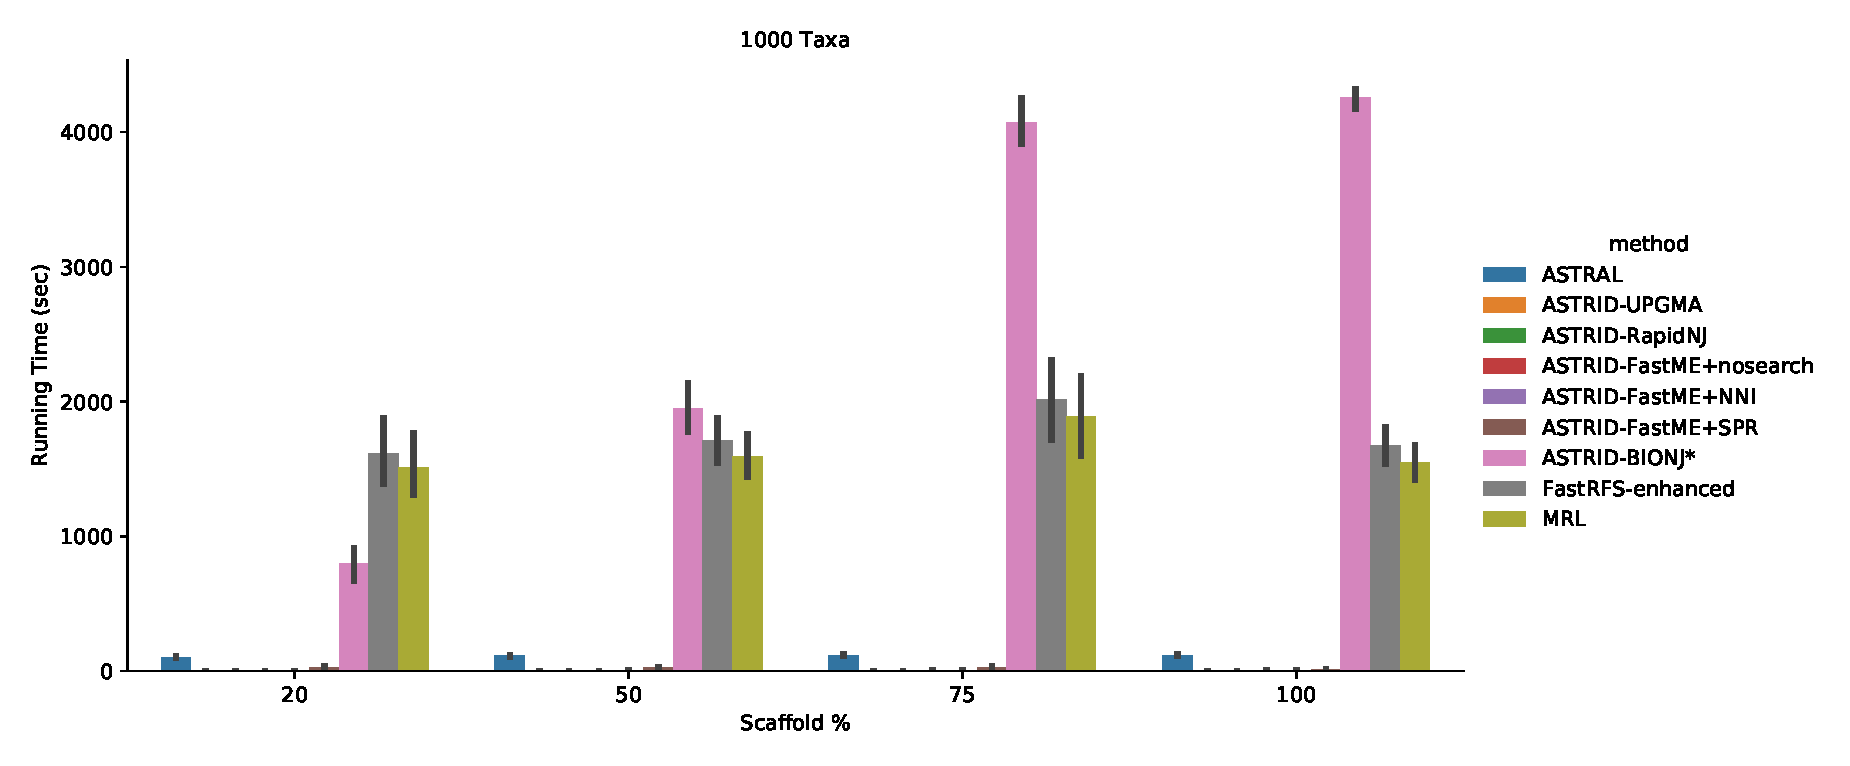
\includegraphics[width=\textwidth]{astrid-missing-figs/running-times-all.eps}
    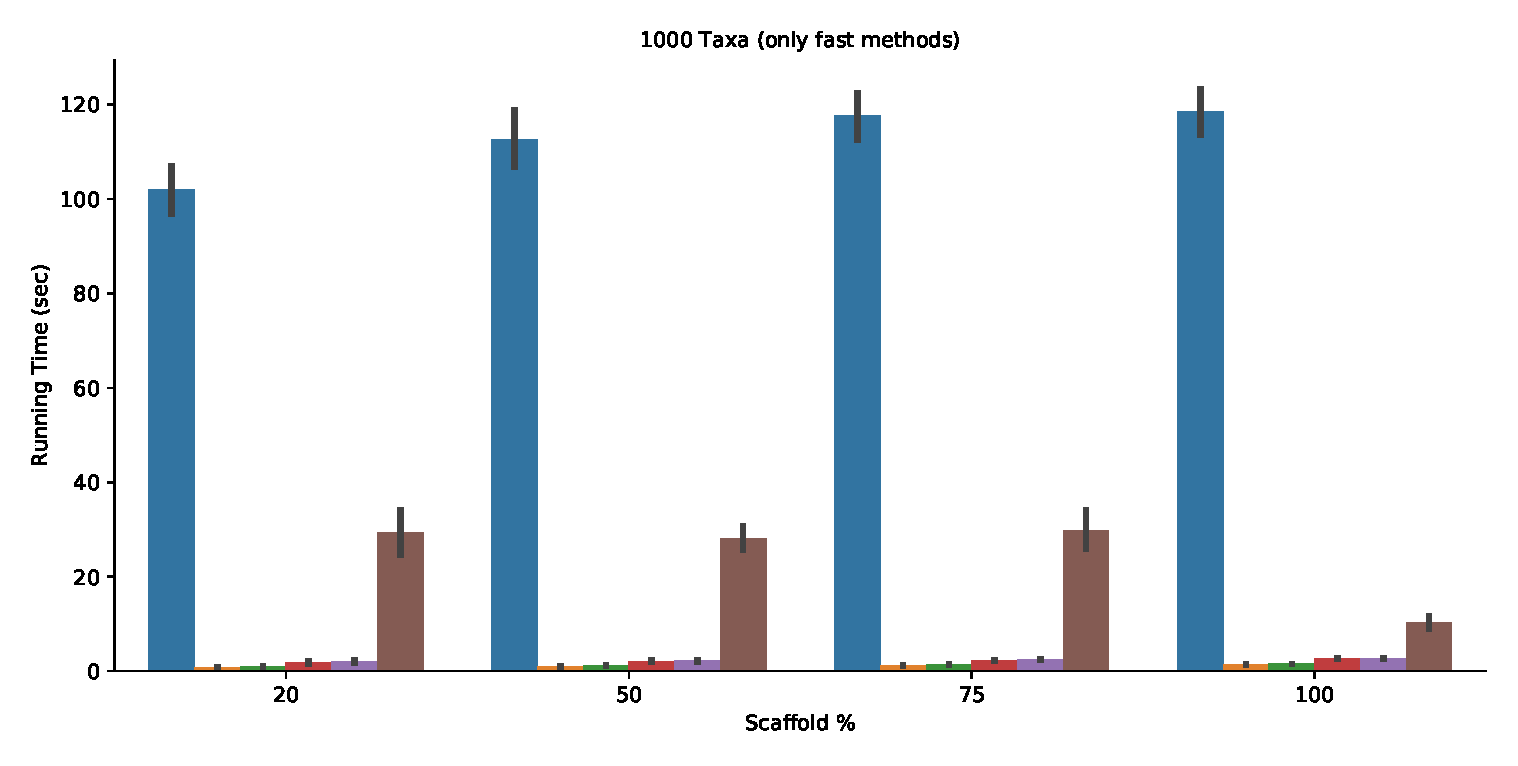
\includegraphics[width=\textwidth]{astrid-missing-figs/running-times-fast.eps}
    \caption[Running times for supertree methods on simulated SMIDgen data]{Comparison of running times for supertree methods on simulated SMIDgen data with 1000 taxa and 16 source trees. Data is averaged over 10 replicates. The second figure shows the same data, but without the slowest methods (MRL, FastRFS, ASTRID-BIONJ*). Calculations were run on a 16-core AMD Interlagos Blue Waters node with 64 GB RAM; FastME, ASTRAL and the ASTRAL subroutines in FastRFS are multithreaded.}
    \label{astrid-missing::fig:running-times}
\end{figure*}


\begin{table*}[htb!]
    \centering
\begin{tabular}{llrrrrrrrrr}
\hline
     &  &  ASTRAL &    MRL &  FastRFS-enhanced &  \makecell{ASTRID\\UPGMA} &  \makecell{ASTRID\\BIONJ*} &  \makecell{ASTRID\\RapidNJ} &  \makecell{ASTRID\\FastME\\+nosearch} &  \makecell{ASTRID\\FastME\\+NNI} &  \makecell{ASTRID\\FastME\\+SPR} \\
Taxa & Scaffold \% &         &        &                   &               &                &                 &                         &                    &                    \\

100  & 20  &     6.3 &    7.7 &              11.1 &           0.0 &            4.6 &             0.0 &                     0.0 &                0.0 &                0.0 \\
     6 trees & 50  &     6.5 &    7.7 &              11.2 &           0.0 &            5.0 &             0.0 &                     0.0 &                0.0 &                0.0 \\
     & 75  &     6.5 &    8.0 &              11.6 &           0.0 &            6.2 &             0.0 &                     0.0 &                0.0 &                0.0 \\
     & 100 &     7.1 &    7.7 &              11.2 &           0.0 &            4.7 &             0.0 &                     0.0 &                0.0 &                0.0 \\
     \hline
{500}  & 20  &    40.4 &  270.0 &             296.6 &           0.2 &          140.0 &             0.2 &                     0.3 &                0.3 &                3.0 \\
     11 trees& 50  &    42.6 &  288.0 &             317.7 &           0.2 &          239.0 &             0.2 &                     0.4 &                0.4 &                3.0 \\
     & 75  &    44.1 &  321.8 &             353.6 &           0.2 &          556.6 &             0.3 &                     0.4 &                0.5 &                3.2 \\
     & 100 &    46.5 &  290.4 &             322.0 &           0.3 &          504.4 &             0.3 &                     0.5 &                0.5 &                1.4 \\
     \hline
{1000} & 20  &   102.0 & 1510.4 &            1615.4 &           0.7 &          799.4 &             0.9 &                     1.8 &                2.0 &               29.4 \\
 16 trees    & 50  &   112.6 & 1589.8 &            1708.8 &           0.9 &         1947.9 &             1.2 &                     2.1 &                2.2 &               28.1 \\
     & 75  &   117.7 & 1888.6 &            2014.1 &           1.1 &         4074.3 &             1.3 &                     2.3 &                2.5 &               29.7 \\
     & 100 &   118.5 & 1548.5 &            1676.4 &           1.3 &         4259.1 &             1.5 &                     2.6 &                2.7 &               10.2 \\
\end{tabular}
     \caption[Running times (in seconds) for ASTRID variants and supertree methods on SMIDgen simulated data]{Comparison of running times (in seconds) for ASTRID variants and supertree methods on SMIDgen simulated data. 100- and 500-taxon datasets had 30 replicates per model condition, and 1000-taxon datasets had 10 replicates per model condition. Time for FastRFS includes time to run MRL for the expanded search space. Some methods took less than 0.05 seconds on average on the 100-taxon datasets; these are listed as taking 0.0 seconds to complete. Calculations were run on a 16-core AMD Interlagos Blue Waters node with 64 GB RAM; FastME, ASTRAL and the ASTRAL subroutines in FastRFS are multithreaded. }
    \label{astrid-missing::tab:runningtimes}
\end{table*}
   

\section{Results}


\subsection{Determining the best way to run ASTRID}

The first set of experiments varied the parameters for ASTRID to determine the best way to run it. In addition to testing the previous version of ASTRID, which used BIONJ*, we tested the iterative protocol with FastME with no searches, FastME+NNI, FastME+SPR, and RapidNJ for the second stage. We tested the iterative protocol with up to three iterations of the second-stage method to determine if more iterations improved the results.

\subsubsection{Number of iterations}

We first compare running multiple iterations of FastME with no local search, NNIs, or NNIs and SPRs (see Fig. \ref{astrid-missing::fig:iterations-err}). 

These experiments show that additional iterations of FastME beyond the first do not improve the results for any of the FastME search types; in fact, there was never any difference between the number of iterations. However, there was a significant extra running time cost for additional iterations, especially for ASTRID-FastME+SPR, where the running time was dominated by the cost to run the distance method.

Therefore, for the remainder of the experiments, we only used a single iteration of the second stage distance methods.



\subsubsection{FastME local search variants}

FastME with no local search is typically less accurate than using NNIs and SPRs (see Fig. \ref{astrid-missing::fig:iterations-err}). FastME+SPR is always at least as accurate as FastME+NNI, and in some cases is slightly more accurate (see Fig. \ref{astrid-missing::fig:astrid-bionj-errs}). This difference was most pronounced on the 20\% scaffold datasets.

NNIs take essentially zero additional time, but SPRs come at a significant running time cost, as seen in Table \ref{astrid-missing::tab:runningtimes} and Fig. \ref{astrid-missing::fig:running-times}. On the 1000 taxon datasets,  ASTRID with a single iteration of FastME+NNI completed in between 1 and 3 seconds on every replicate, whereas ASTRID with a single iteration of FastME+SPR took between 18 and 43 seconds on the 20\%, 50\%, and 75\% scaffold datasets; and between 7 and 15 seconds on the 100\% scaffold datasets.

For the remainder of the analyses in this study, we will not show results run with more than one iteration of FastME, and we will only show the FastME-NNI and FastME-SPR variants of FastME.


\subsubsection{Other distance methods}

Earlier versions of ASTRID used BIONJ* as its distance method in the cases where the distance matrix was missing entries. Figure \ref{astrid-missing::fig:astrid-bionj-errs} shows that the new UPGMA protocol with FastME significantly reduces the error rate under the model conditions where BIONJ* returns inaccurate trees.

We also experimented with RapidNJ as the distance method for the second stage of the UPGMA protocol; its accuracy is better than UPGMA* alone or BIONJ*, but not as good as either FastME variant. It was, however, faster than FastME, taking an average of between 0.9 and 1.5 seconds on the 1000-taxon model conditions, while FastME with no local search took between 1.8 and 2.6 seconds.

Furthermore, Table \ref{astrid-missing::tab:runningtimes} and Figure \ref{astrid-missing::fig:running-times} show that the UPGMA protocol has a huge improvement in running time. For example, on the 75\% scaffold 1000-taxon data, ASTRID-BIONJ* took an average of 1 hour 7 minutes, while ASTRID-FastME+NNI took just 2.5 seconds and ASTRID-FastME+SPR took 30 seconds. ASTRID-RapidNJ was slightly faster than ASTRID-FastME+NNI, and ASTRID-UPGMA was (by nature) faster than the rest.

\subsection{Comparison to ASTRAL and supertree methods}

ASTRID's accuracy is comparable to ASTRAL's, as seen in \ref{astrid-missing::fig:astral-errs}. On the $20\%$ scaffold datasets, ASTRAL performed slightly better than ASTRID. However, ASTRAL is somewhat slower than ASTRID-FastME+SPR, and much slower than ASTRID-FastME+NNI, as shown in Table \ref{astrid-missing::tab:runningtimes} and Figure \ref{astrid-missing::fig:running-times}.

MRL also has a similar accuracy to ASTRAL and ASTRID; it is, however, substantially slower than both of them, taking over 30 minutes to run on the 1000-taxon datasets that require 2 minutes for ASTRAL, 30 seconds for ASTRID-FastME+SPR, and under 3 seconds for ASTRID-FastME+NNI. 

FastRFS is slightly more accurate than ASTRAL and ASTRID, but takes approximately as long as MRL to run, since the majority of its running time is taken by running MRL to enhance FastRFS's search space.




\subsection{Scalability to very large datasets}

On the large 43,183 taxon RNAsim dataset, ASTRAL failed to complete. It ran out of memory on a computer with 256GB RAM before even computing its constraint set. Since FastRFS requires ASTRAL's constraint set to run, it too was not able to run on this dataset.

ASTRID-RapidNJ was able to complete extremely quickly on this dataset, running in just 25 minutes with 110GB RAM. However, its error was quite high, at 55\%. 

ASTRID-FastME (no search) was slower, taking 4 hours 22 minutes and 132GB RAM. Its error was 26\%. 

ASTRID-FastME+NNI was slightly slower, at 5 hours 42 minutes, and also required 132GB RAM. Its error was lower, at 23\%.

ASTRID-FastME+SPR also ran out of memory.

MRL with FastTree was able to run, and only required 29GB of RAM. However, it was much slower, taking 24 hours 17 minutes to complete, and had higher error than ASTRID-FastME+NNI, at 31\%.

\begin{table*}[]
    \centering
\begin{tabular}{l|rrr}
     Method & Running Time (HH:MM) & Memory usage (GB) & RF Error\\
    \hline
     ASTRID-RapidNJ & 00:25 & 110 & 55\%\\
     ASTRID-FastME & 04:22 & 132 & 26\% \\
     ASTRID-FastME+NNI & 05:42 & 132 & 23\% \\
     MRL-FastTree & 24:17 & 29 & 31\%
\end{tabular}
\caption[Running times and memory usage for 43,183 taxon simulated RNAsim-based dataset]{Running times and memory usage for 43,183 taxon simulated RNAsim-based dataset with 31 source trees. Source trees were simulated by sampling clade-based and scaffold trees from a 50,000 taxon RNAsim tree. FastRFS, ASTRAL, and MRL-RAxML were not able to run due to excessive memory usage. Calculations were run on a 20-core Intel Ivy Bridge cluster node with 256GB RAM; FastME, ASTRAL and the ASTRAL subroutines in FastRFS are multithreaded.}
\label{astrid-missing::tab:rnasim-runningtime}
\end{table*}


\subsection{Biological dataset}
On the 2,228 taxon CPL biological dataset with 39 source trees, we report running time and memory usage in Table \ref{astrid-missing::tab:cpl-runningtime}. ASTRID-FastME+NNI was by far the fastest method, completing in just 13 seconds and requiring only 489MB RAM. ASTRAL was faster than ASTRID-FastME+SPR, but had much higher RAM usage (over 8GB) than any of the other methods. ASTRID-BIONJ* was much slower than the rest of the methods, requiring nearly six hours to run.

On the two smaller biological datasets, running times and memory usage are shown in Tables \ref{astrid-missing::tab:thpl-runningtime} and \ref{astrid-missing::tab:seabirds-runningtime}. On the 121-taxon seabird dataset, no method took more than a few seconds to complete. On the 558-taxon THPL dataset, FastRFS took 13 minutes, ASTRID-BIONJ* took just over 1 minute, arunnd ASTRAL and the iterative ASTRID variants completed in a few seconds.

On all these datasets, ASTRAL and ASTRID-BIONJ* had substantially higher memory usage requirements than the rest of the methods. This may be due to the fact that ASTRAL and BIONJ* are implemented in Java, while the rest of the methods are implemented in C or C++. 

\begin{table*}[hbt!]
    \centering
\begin{tabular}{l|rr}
     Method & Running Time (HH:MM:SS) & Memory usage (MB)\\
    \hline
     ASTRID-BIONJ* & 5:47:00 & 8598 \\
     ASTRID-FastME+NNI & 00:00:13 & 489 \\
     ASTRID-FastME+SPR & 00:12:30 & 746 \\
     ASTRAL & 00:01:02 & 5200 \\
     FastRFS & 00:04:15 & 353 \\
\end{tabular}
\caption[Running times and memory usage for 2228-taxon comprehensive papilinoid legume (CPL) dataset]{Running times and memory usage for 2228-taxon comprehensive papilinoid legume (CPL) dataset with 39 trees \cite{wojciechowski2000molecular}. FastRFS was run without MRL enhancement tree. Calculations were run on a 20-core Intel Ivy Bridge cluster node with 256GB RAM; FastME, ASTRAL and the ASTRAL subroutines in FastRFS are multithreaded.}
\label{astrid-missing::tab:cpl-runningtime}
\end{table*}

\begin{table*}[hbt!]
    \centering
\begin{tabular}{l|rr}
     Method & Running Time  (HH:MM:SS) & Memory usage (MB)\\
    \hline
     ASTRID-BIONJ* & 00:00:04 & 80 \\
     ASTRID-FastME+NNI & 00:00:00 & 6.9 \\
     ASTRID-FastME+SPR & 00:00:00 & 7.4 \\
     ASTRAL & 00:00:02 & 408 \\
     FastRFS & 00:00:01 & 3.6 \\
\end{tabular}
\caption[Running times and memory usage for 121-taxon seabirds dataset]{Running times and memory usage for 121-taxon seabirds dataset \cite{kennedy2002seabird}. FastRFS was run without MRL enhancement tree. Calculations were run on a 20-core Intel Ivy Bridge cluster node with 256GB RAM; FastME, ASTRAL and the ASTRAL subroutines in FastRFS are multithreaded.}
\label{astrid-missing::tab:seabirds-runningtime}
\end{table*}

\begin{table*}[hbt!]
    \centering
\begin{tabular}{l|rr}
     Method & Running Time  (HH:MM:SS) & Memory usage (MB)\\
    \hline
     ASTRID-BIONJ* & 00:01:12 & 1108 \\
     ASTRID-FastME+NNI & 00:00:00 & 32 \\
     ASTRID-FastME+SPR & 00:00:06 & 52 \\
     ASTRAL & 00:00:06 & 2351 \\
     FastRFS & 00:13:00 & 24 \\
\end{tabular}
\caption[Running times and memory usage for 558-taxon temperate herbaceous papilinoid legume (THPL) dataset]{Running times and memory usage for 558-taxon temperate herbaceous papilinoid legume (THPL) dataset \cite{mcmahon2006phylogenetic}. FastRFS was run without MRL enhancement tree. Calculations were run on a 20-core Intel Ivy Bridge cluster node with 256GB RAM; FastME, ASTRAL and the ASTRAL subroutines in FastRFS are multithreaded.}
\label{astrid-missing::tab:thpl-runningtime}
\end{table*}

\section{Discussion}

Supertree estimation is an important tool for next generation phylogenomic analyses. The development of accurate supertree methods that can scale to datasets with tens or hundreds of thousands of taxa is critical for these projects. Existing state-of-the-art methods can scale to datasets with thousands of taxa, but struggle to go beyond that due to running time and memory utilization constraints. 

The improved version of ASTRID presented here can perform analyses much larger than existing supertree methods. ASTRID's most significant advantage in the supertree context is its ability to scale to extremely large datasets while maintaining a low error rate. In particular, when the number of input trees is relatively low compared to the number of taxa, ASTRID's running time is dominated by the distance method used. This improved version of ASTRID allows fast distance methods to be used even in the supertree context when the ASTRID distance matrix is missing entries.

ASTRID-FastME+SPR is the most accurate version of ASTRID, and should be used if running time and memory constraints allow. However, the asymptotic runtime of the SPR step is $O(n^3)$, and the memory usage is empirically higher than with just NNIs, so scaling this technique beyond a few thousand taxa is unlikely.

ASTIRD-FastME+NNI is slightly less accurate than ASTRID-FastME+SPR under some conditions, but substantially faster and memory-efficient. It can scale to datasets with tens of thousands of taxa while maintaining low error rates. 

For even larger datasets, ASTRID-RapidNJ may be able to scale beyond the level of FastME. However, it it is less accurate than FastME, so it is not usually the best method to use.

\section{Conclusions}

We have presented an improved version of ASTRID that significantly improves performance, in terms of accuracy and running time, in the supertree context. We have explored several ways to run ASTRID on a variety of datasets, and compared its performance to other leading methods, including ASTRAL, FastRFS, or MRL. ASTRID is competitive in terms of accuracy with these methods, and is able to scale to very large datasets that cannot be analyzed with any other method. 

ASTRID allows for a variety of distance methods to be used, with slower but more accurate methods like FastME+SPR ideal for small to medium sized datasets, and faster methods like FastME+NNI and RapidNJ allowing for scaling to datasets with tens of thousands of taxa.

\subsection{Future work}

It is likely possible to further optimize ASTRID to limit memory consumption, particularly the built-in UPGMA* implementation. Some distance methods, including RapidNJ, are able to scale to extremely large datasets by intelligently storing data to disk when the entire distance matrix would not fit into memory. It may be possible to implement a similar approach in ASTRID, which would enable virtually limitless scaling.

Additional improvements to the distance methods used by ASTRID could also improve its performance. For example, it may be possible to directly add support for incomplete distance matrices to FastME. There may also be better methods than UPGMA* for the first stage of the ASTRID iterative protocol. 

  \subsection{Additional figures}
\begin{figure}
    \centering
    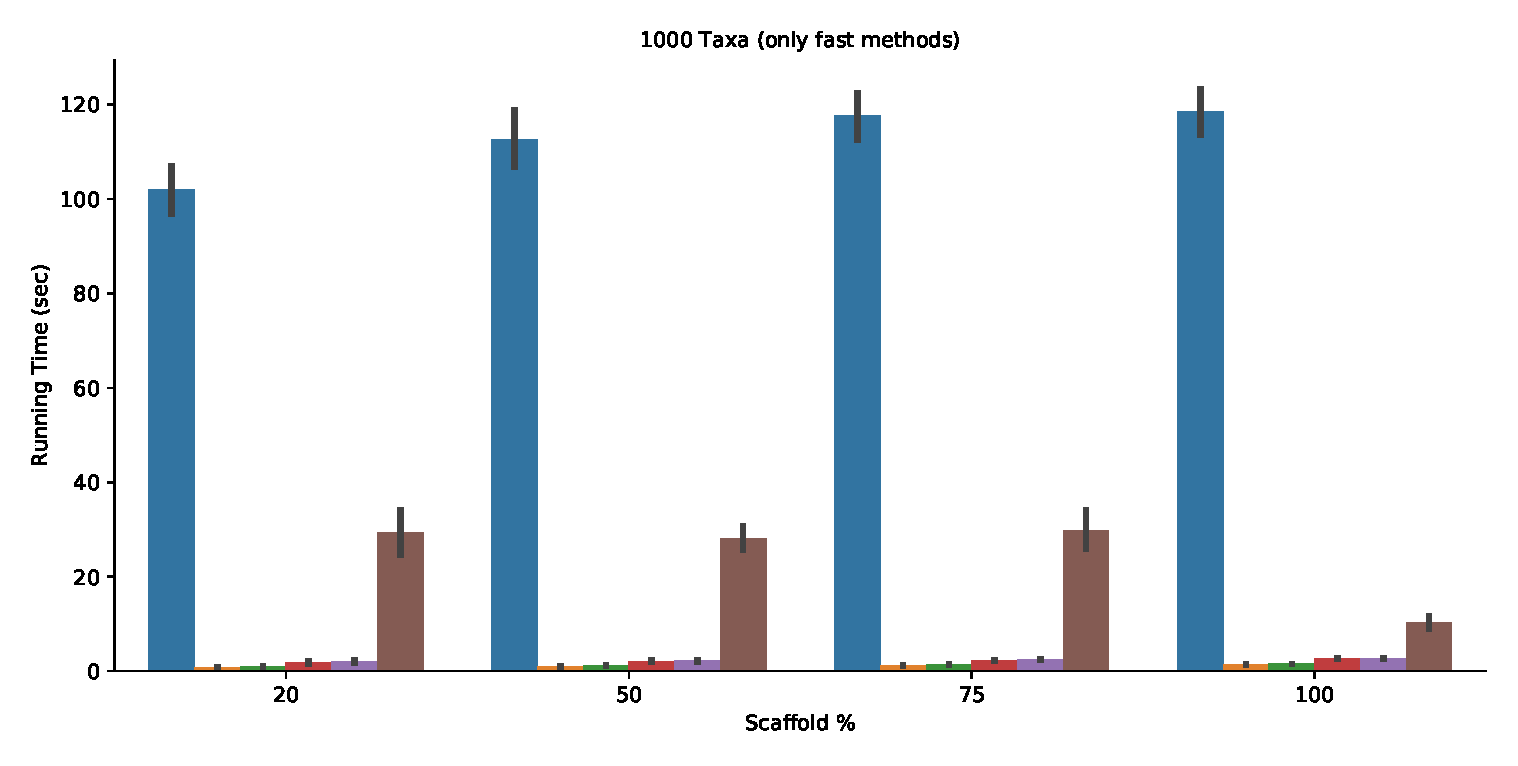
\includegraphics[width=\textwidth]{astrid-missing-figs/running-times-fast.eps}
    \caption{RF Error for 1000-taxon simulated datasets using up to 3 iterations of FastME with NNIs and FastME with SPRs. Each model condition has 10 replicates.}
    \label{astrid-missing::fig:iterations-err}
\end{figure}


\begin{figure}
    \centering
    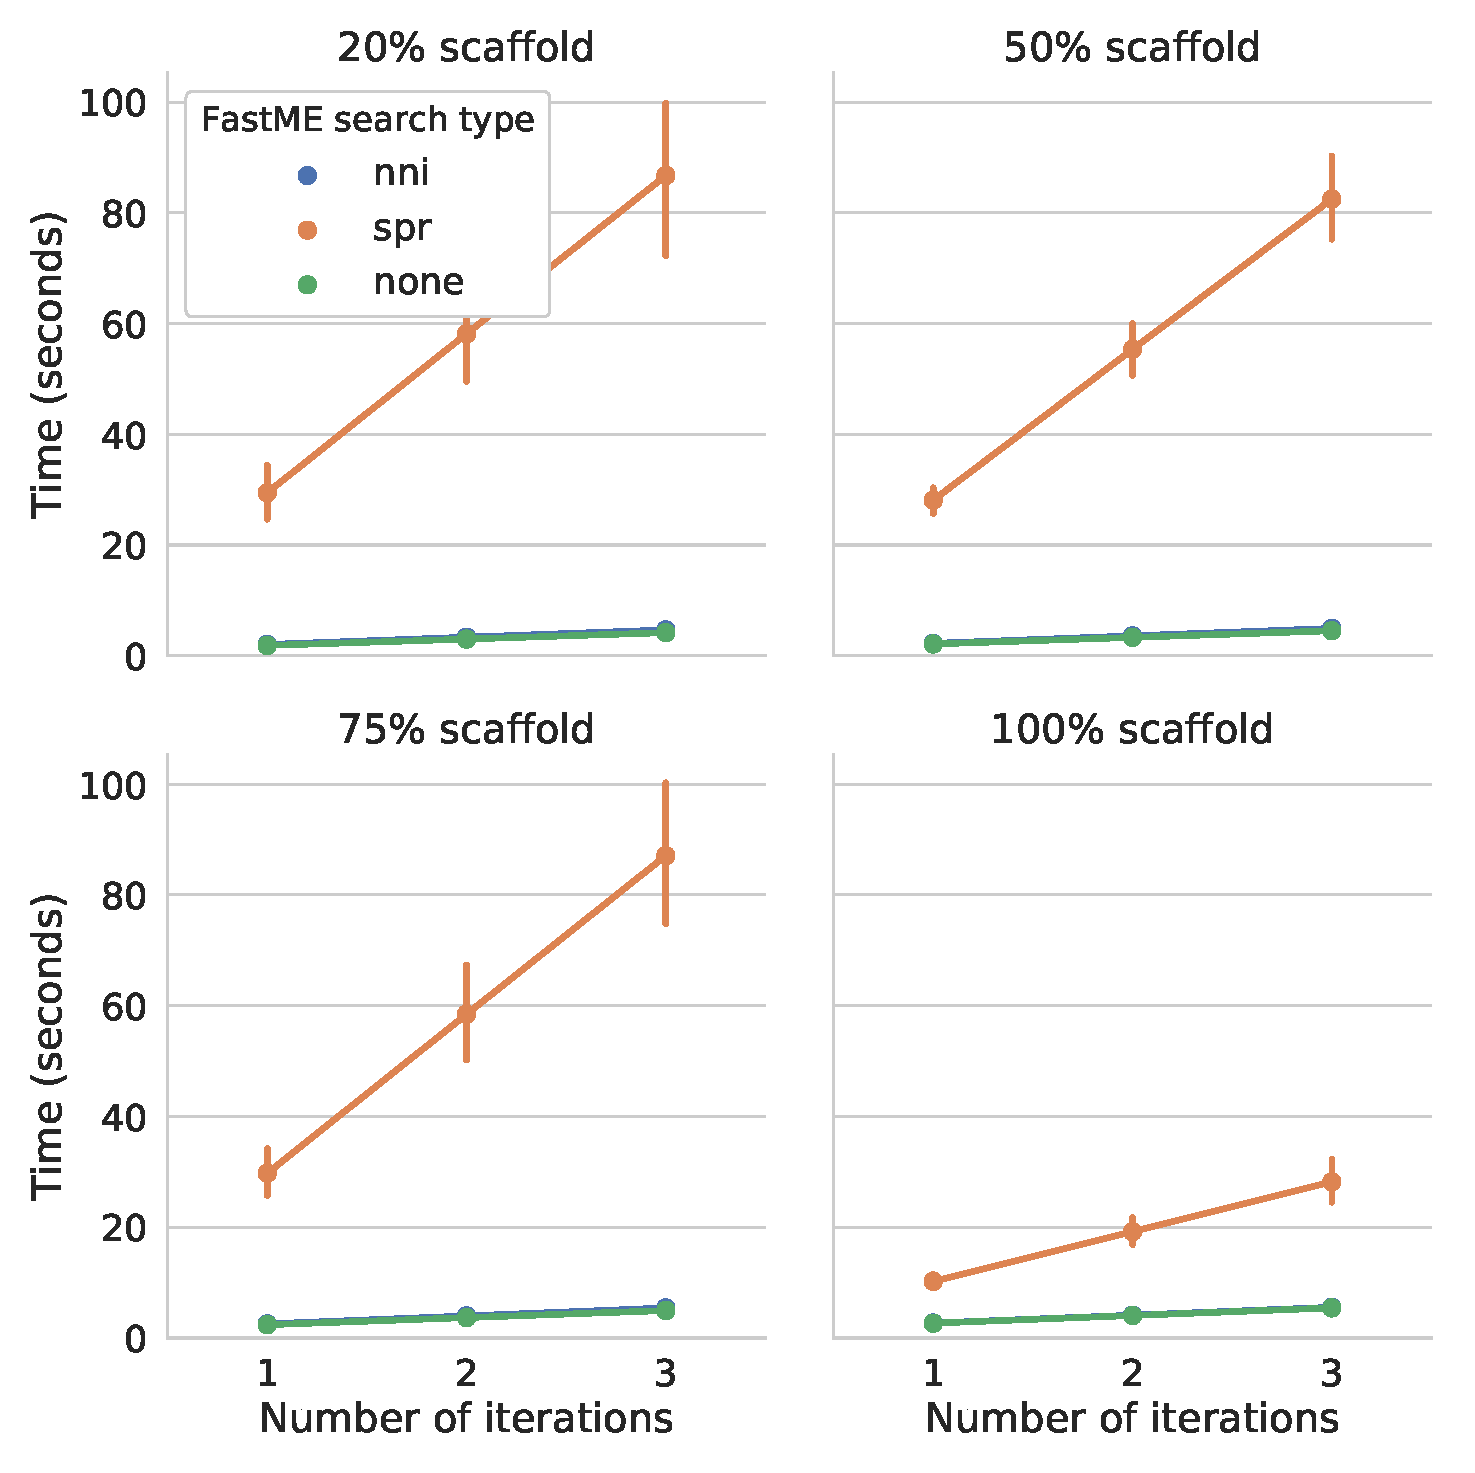
\includegraphics[width=\textwidth]{astrid-missing-figs/iterations-times.eps}
    \caption{Running times for 1000-taxon simulated datasets using up to 3 iterations of FastME with NNIs and FastME with SPRs. Each model condition has 10 replicates.}
    \label{astrid-missing::fig:iterations-times}
\end{figure}